\documentclass[10pt]{article}

\usepackage[margin = .8in]{geometry}
\usepackage{amsfonts,amsmath,amssymb}
\usepackage{authblk}
\usepackage{bbm}
\usepackage[inline]{enumitem}
\usepackage{graphicx}
\graphicspath{{./}{../image/}}
\usepackage[colorlinks=true,citecolor=blue,urlcolor=blue]{hyperref}
\usepackage{natbib}
\usepackage{setspace}
\setstretch{1.2}


\newcommand{\EE}{{\mathbb{E}}}
\newcommand{\PP}{{\mathbb{P}}}
\newcommand{\QQ}{{\mathbb{Q}}}
\newcommand{\Fb}{\mathbf{F}}
\newcommand{\Ib}{\mathbf{I}}
\newcommand{\hb}{\mathbf{h}}
\newcommand{\xb}{\mathbf{x}}
\newcommand{\one}{\mathbbm{1}}
\newcommand{\Ocal}{\mathcal{O}}


\begin{document}


\title{Progress Report: Transformer-CRF Integration for Sequence Labeling on
EEG Data}

\author[1]{Xiaohang Ma}
\author[2]{Shiying Xiao}
\author[2]{Xiaohui Yin}

\affil[1]{Department of Mathematics, University of Connecticut}
\affil[2]{Department of Statistics, University of Connecticut}

\date{\today}

\maketitle


\section{Progress}
% Overview of progress made and key accomplishments.


The project is progressing according to schedule. To date, we have made
significant strides in several key areas:
\begin{enumerate}
\item Model Development:
We have initiated development of a convolutional neural network (CNN) combined
with a hidden conditional random field (HCRF). This hybrid approach aims to
create a robust sequence labeling framework capable of capturing both local
and global dependencies within the data sequences.
\item Variational Inference Implementation:
To efficiently approximate the posterior distributions in our complex model,
we have integrated variational inference into the HCRF component.
This technique is particularly effective in handling the computational
challenges posed by the dataset's heterogeneity.
\item Data Visualization:
We have successfully visualized key features of the dataset.
\end{enumerate}
%This progress has provided a foundation for the next
%steps of our research.


\section{Preliminary Results}
% Summary of initial findings and analyses.


The potential of our HCRF model:
\begin{equation*}
\Phi(y, \hb, \xb; \theta) = \underbrace{
\sum_{j \in \nu} \phi(h_j, x_j; \omega) +
\sum_{i \neq j} \psi(h_i, h_j, x_i, x_j; \eta)}_{
% \propto \log\PP ( \hb \vert \xb; \theta)
\textrm{Measures log-likelihood $\log\PP ( \hb \vert \xb; \theta)$}}
+ \underbrace{
\sum_{j \in \nu} \varphi(y, h_j, x_j; \delta) +
\vartheta(y, \xb; \varpi)}_{
% \propto \log \PP (y | \hb,  \xb; \theta)
\textrm{Measures log-likelihood $\log \PP (y \vert \hb, \xb; \theta)$}}
\end{equation*}


\begin{itemize}
\item \textbf{Unary Potential} $\phi(h_j, x_j; \omega)$ measures
the likelihood of the local feature $x_j$ is assigned as
the hidden attention state $h_j$.
We generate the likelihood through a softmax operation on $\Fb(\xb)$
the feature maps of CNN with $(N, C_{\textrm{out}})$ dimensions,
by which the potential of each pixel $x_j$ assigned as each state of
hidden state set $\{0, 1, \dots, 5\}$
is drawn and represented by a matrix with $(N, 2)$ dimension.
\item The parameter $\omega$ is learned by our end-to-end CNN-Unet training 
structure.
\item \textbf{Unary Potential} $\varphi(y, h_j; \delta)$ measures
the compatibility between global class label $y$ and the hidden local
state $h_j$. This potential is parametrized as:
\begin{align*}
\varphi(y, h_{j}; \delta) = \sum_{a \in Y} \sum_{b \in H} \delta_{a, b}
\cdot \one(y = a) \cdot \one(h_j = b).
\end{align*}
\item \textbf{Binary Potential} $\psi(h_i, h_j, x_i, x_j; \eta)$
balances the hidden label compatibility of the neighboring pixels on the 
feature image $\Fb(\Ib)$.
We define this potential through a common contrast-sensitive two-kernal 
potentials (see~\citet{krahenbuhl2011efficient} and \citet{chen2022end}):
\begin{equation*}
\psi(h_i, h_j, x_i, x_j; \eta) = \mu(h_i, h_j) \Bigg[
\omega_1 \exp \left(
-\frac{\left\lvert p_i - p_j \right\rvert^2}{2\eta_\alpha^2}-
-\frac{\left\lvert \Fb_i(\Ib) - \Fb_j(\Ib) \right\rvert^2}{2\eta_\beta^2} 
\right) + \omega_2 \exp \left(
- \frac{\left\lvert p_i - p_j \right\rvert^2}{2 \eta_\gamma^2}
\right)
\Bigg]
\end{equation*}
\end{itemize}


While the models are still under development and optimization,
initial results are promising. For instance, Figure~\ref{fig:SEIZURE_3}
illustrates a sample prediction with ground truth 94.\% Seizure and 2.9\% LPD.
Our model predicts 88.4\% Seizure and 1.6\% LPD.
Yellow highlights indicate the regions where the model focused its attention.
These preliminary results show trends that are consistent with our initial
hypotheses. The visualizations have proven useful in pinpointing areas for
further investigation, and the derived formulas appear to be robust and
aligned with the expected model outcomes. Further analysis will refine
these findings and explore additional dimensions of data.


\begin{figure}[tbp]
\centering
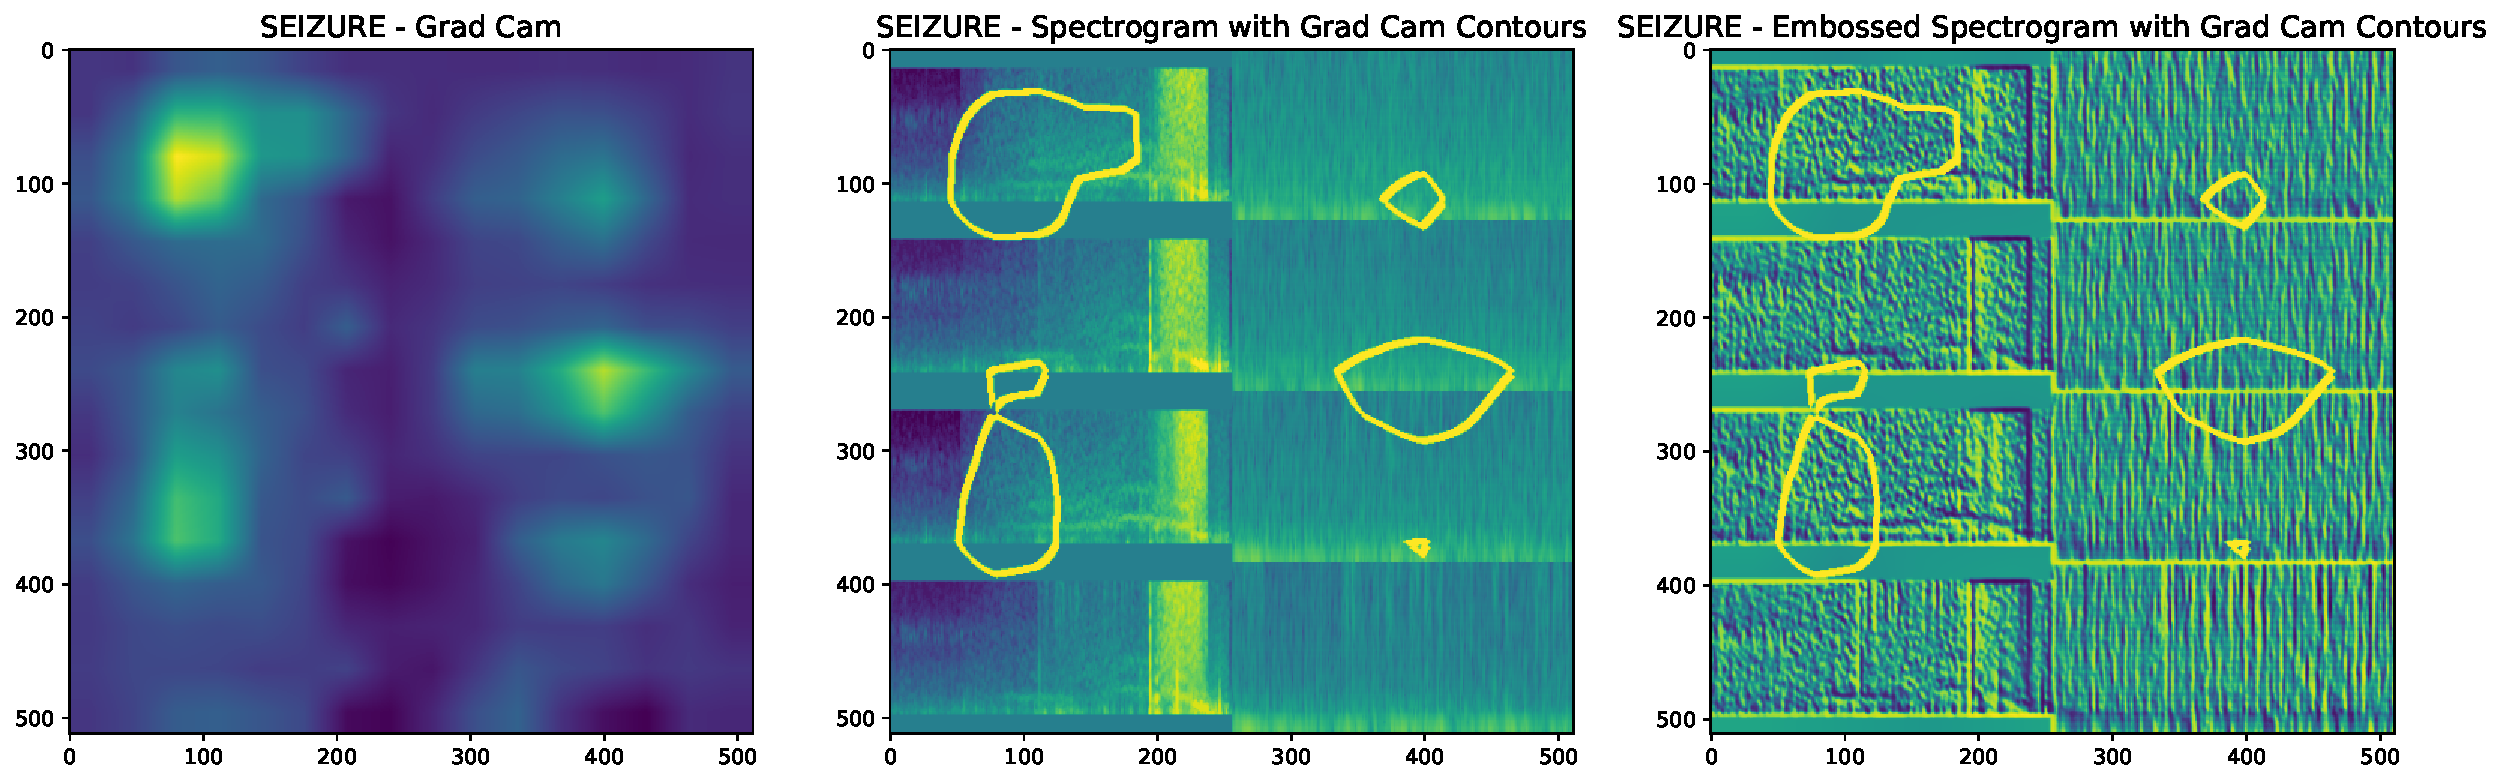
\includegraphics[width=.8\textwidth]{grad_cam_SEIZURE_3}
\caption{An example of data visualization. Areas highlighted in yellow
indicate regions where the model focused its attention during this specific
prediction.}
\label{fig:SEIZURE_3}
\end{figure}


\section{Challenges}
% Discussion of any challenges faced during the project.


We encountered minor challenges related to data handling and computational
limitations. In particular, the complexity of certain calculations required
additional processing time, which slightly delayed our progress.
We are currently exploring ways to optimize these computations.


\section{Plan Changes}
% Outline of any adjustments made to the original plan.


At this stage, we have not made significant changes to our original plan.
However, due to the complexity of the dataset and model, we may consider
slightly adjust the project timeline to allocate additional time for
model fine-tuning.


\section{Next Steps}
% Description of remaining tasks and strategy for completion.


The remaining tasks include:
\begin{enumerate*}[label = (\roman*)]
\item Expanding and refining the visualizations based on updated data.
\item Finalizing the derivation and validation of all essential formulas.
\item Conducting a comprehensive analysis with the refined model.
\item Preparing the final report and presentation materials.
\end{enumerate*}


\section{Updates}
% Additional relevant updates or future directions.


We will provide regular updates on model performance, challenges encountered,
and any significant changes to the project plan.

%\section{CNN-HCRF Model}
%
%The classical hidden conditional random field (HCRF) model can be formulated as
%\begin{align}
%\PP(y \vert \xb; \theta) &= \sum_{\hb \in H^N}
%\mathbb{P}(y, \hb \vert \xb; \theta) \\
%&= \frac{\sum_{\hb \in H^N} \exp\left(\Phi(y, \hb, \xb; \theta)\right)}
%{\sum_{y^\prime} \sum_{\hb \in H^N}
%	\exp\left(\Phi(y^\prime, \hb, \xb; \theta)\right)}.
%\end{align}
%
%
%Different to the design of most existing HCRF models, which they assign
%potentials based on the features predefined from the input data $\Ib$.
%% \( \PP(y, \hb \vert \xb; \theta) \).
%%  Here, we consider a generative model that constructing
%% \( \PP(\hb \vert \xb; \theta) \) through a CRF framework then using an 
%%unary potential for , 
%Our HCRF replace $I$ with features learned by CNN, \(i.e. \ 
%\Fb(\Ib)\). 
%Thus the new potentials become:
%\begin{align*}
%\Phi(y, \hb, \xb; \theta) = \Phi(y, \hb, \Fb(\Ib); \theta).
%%\PP (y, \hb \vert \xb; \theta) = \PP (y \vert \hb, \xb; \theta)
%%\cdot \PP ( \hb \vert \xb; \theta).
%\end{align*}
%Thus, we design the potential of our HCRF model as.
%\begin{align}
%\Phi(y, \hb, \xb; \theta) & = \underbrace{
%\sum_{j \in \nu} \phi(h_j, x_j; \omega) +
%\sum_{i \neq j} \psi(h_i, h_j, x_i, x_j; \eta)}_{
%% \propto \log\PP ( \hb \vert \xb; \theta)
%\textrm{Measures log-likelihood $\log\PP ( \hb \vert \xb; \theta)$}} \\
%& + \underbrace{
%\sum_{j \in \nu} \varphi(y, h_j, x_j; \delta) +
%\vartheta(y, \xb; \varpi)}_{
%% \propto \log \PP (y | \hb,  \xb; \theta)
%\textrm{Measures log-likelihood $\log \PP (y \vert \hb, \xb; \theta)$}}
%\end{align}
%
%
%{\textbf{Unary Potential}} $\phi(h_j, x_j; \omega)$: measures
%the likelihood of the local feature $x_j$ is assigned as
%the hidden attention state $h_j$.
%We generate the likelihood through a softmax operation on $\Fb(\xb)$
%the feature maps of CNN with $(N, C_{\textrm{out}})$ dimensions,
%by which the potential of each pixel $x_j$ assigned as each state of
%hidden state set $\{0, 1, \dots, 5\}$
%is drawn and represented by a matrix with $(N, 2)$ dimension.
%
%The parameter $\omega$ is learned by our end-to-end CNN-Unet training 
%structure.
%
%
%{\textbf{Unary Potential}} $\varphi(y, h_j; \delta)$ measures
%the compatibility between global class label $y$ and the hidden local
%state $h_j$. This potential is parametrized as:
%\begin{align*}
%\varphi(y, h_{j}; \delta) = \sum_{a \in Y} \sum_{b \in H} \delta_{a, b}
%\cdot \one(y = a) \cdot \one(h_j = b).
%\end{align*}
%
%
%{\textbf{Binary Potential}} $\psi(h_i, h_j, x_i, x_j; \eta)$
%balances the hidden label compatibility of the neighboring pixels on the 
%feature image $\Fb(\Ib)$.
%We define this potential through a common contrast-sensitive two-kernal 
%potentials see~\citet{krahenbuhl2011efficient} and \citep{chen2022end}:
%
%
%\begin{equation}
%\begin{split}
%\psi(h_i, h_j, x_i, x_j; \eta) = \mu(h_i, h_j) \Bigg[
%& \omega_1 \exp \left(
%-\frac{\left\lvert p_i - p_j \right\rvert^2}{2\eta_\alpha^2}-
%-\frac{\left\lvert \Fb_i(\Ib) - \Fb_j(\Ib) \right\rvert^2}{2\eta_\beta^2} 
%\right) \\
%& + \omega_2 \exp \left(
%- \frac{\left\lvert p_i - p_j \right\rvert^2}{2 \eta_\gamma^2}
%\right)
%\Bigg]
%\end{split}
%\end{equation}
%
%
%
%\section{Variational Inference of HCRF}
%
%
%\subsection{ELBO Under Mean-Filed Variational Family}
%
%
%The existence of the hidden variable $\hb$ makes our model more 
%interpretable. However, since We will train our model through maximal 
%likelihood method, 
%introducing the hidden variable will make precisely computation the summation 
%$\sum_{\hb \in H^N} \PP(y, \hb \vert \xb; \theta)$ intractable.
%To address this issue, we make our computation more feasible through a 
%mean-field variational inference framework, which enables our model 
%efficiently 
%estimating the log-likelihood $\log\PP(y \vert \xb; \theta)$.
%
%
%Firstly, we introduce the mean-field varepsilon family approximation of 
%$\log\PP(\hb \vert y, \xb; \theta)$ as:
%\begin{align*}
%\QQ(\hb) = \prod_{i=1}^N q_i(h_i).
%\end{align*}
%Then the evidence lower bound(ELBO) under the mean-field family is given by
%
%
%\begin{equation}
%\begin{split}
%\textrm{ELBO}(\QQ) &= \EE_{\QQ(\hb)} \log \PP (y, \hb \vert \xb; \theta)
%- \EE_{\QQ(\hb)} \log q(\hb) \\
%& = \sum_{i=1}^N \EE_{q_i(h_i)}
%\left[ \phi(h_j, x_j; \omega) + \varphi(y, h_j, x_j; \delta) \right] \\
%&\quad + \sum_{i=1}^N \sum_{j=1}^N \sum_{l,l^\prime} \one_{\{i \neq j\}} 
%\QQ(h_i = l) \QQ(h_j = l^\prime) \mu(l, l^\prime) \\
%&\qquad \Bigg[ \omega_1 \exp \left(
%- \frac{\left\lvert p_i - p_j \right\rvert^2}{2\eta_\alpha^2}
%- \frac{\left\lvert \Fb_i(\Ib) - \Fb_j(\Ib) \right\rvert^2}{2\eta_\beta^2}
%\right) \\
%&\qquad + \omega_2 \exp \left(
%- \frac{\left\lvert p_i - p_j \right\rvert^2}{2\eta_\gamma^2}
%\right) \Bigg] \\
%&\quad - \sum_{i=1}^N \EE_{q_i} \log q_i(h_i) + \vartheta(y, \xb; \varpi).
%\end{split}
%\end{equation}
%
%
%\subsection{Updating Variational Family}
%
%
%By the coordinate ascent variational inference(CAVI) algorithm, we can obtain 
%that fix \(q_{j}(h_{j}), \forall j \neq i\), the optimal \(q_{i}(h_{i})\) that 
%maximizes \(\textrm{ELBO}(q_{i}(h_{i}))\) is given by
%\begin{align}
%	\mathbb{Q}(h_{i}) \propto \exp\{ \EE_{\mathbb{Q}({\hb_{-i}})} \log 
%	\PP (y, h_{i}, \hb_{-i}|\xb; \theta)\}.
%\end{align}
%
%Thus, we can get that
%\begin{align}
%	q_{i}(l) &= \frac{1}{Z_{i}} \exp \Big\{\phi(h_{j}, x_{j}; \omega) + \varphi
%	(y, h_{j}, x_{j}; \delta) \\
%	& +  \sum_{j\neq i } \sum_{l^{'}}  q(l^{'})\mu(l, l^{'}) 
%	\Big[ \omega_{1} 
%	\exp ( - \frac{\left\lvert p_{i} - p_{j} \right\rvert^{2} }{2 
%	\eta_{\alpha}^{2}}\\
%	&
%	- \frac{\left\lvert \Fb_{i}(\Ib) - \Fb_{j}(\Ib) 
%	\right\rvert^{2} }{2 \eta_{\beta}^{2}})  + \omega_{2}\exp ( - 
%	\frac{\left\lvert p_{i} - p_{j} \right\rvert^{2}}{2 \eta_{\gamma}^{2}})\Big]
%	\Big\}
%\end{align}
%
%
%\subsection{Computational Complexity Analysis}
%
%
%\begin{itemize}
%\item {\textbf{Updating Variational Family}} $\{q_i(h_i)\}$:
%The computationally expensive part of the fixed point iteration of $q_i(h_i)$
%comes from the message passing, \(i.e\). the convolution of $\QQ(\hb)$ and
%gaussian kernal in $\psi(h_i, h_j, x_i, x_j; \eta)$. We need $\Ocal(N^2)$
%runtime for $N$ pixels when evaluating this term precisely.
%To make the computation more feasible, a truncated gaussian kernal will be
%employed, which is only supported on spaces within certain proportion of
%the untruncated standard deviation. Then the approximate message passing is
%linear in the number of pixels $N$.
%\item {\textbf{Computation of the ELBO}}: The summation over the product of 
%$q_i(h_i)q_j(h_j)$ and the gaussian kernal in $\psi(h_i, h_j, x_i, x_j; \eta)$
%also requires a $\Ocal(N^2)$ complexity in time. 
%Owes to a similar truncated gaussian kernal approxiamtion, the runtime can
%be reduced to $\Ocal(N)$.
%\end{itemize}


\bibliography{../manuscript/refs}
\bibliographystyle{chicago}

\end{document}
